\documentclass[11pt,a4paper]{article}
\usepackage{graphicx}
\usepackage{amssymb}
\usepackage[latin1]{inputenc}    %% european characters can be used (Windows, old Linux)
\usepackage[T1]{fontenc}   %% get hyphenation and accented letters right

\pagestyle{empty} % no page numbers
\usepackage[left=35mm, right=35mm, top=15mm, bottom=20mm, noheadfoot]{geometry}

\begin{document}
\thispagestyle{empty}

\title{\textbf{Influencia de rotaci\'on y outflows\\
			    en la l\'inea espectral Lyman Alpha}}
		
\author{Maria Camila Remolina-Gutierrez$^1$, Jaime E. Forero-Romero$^1$\\ \vspace{3mm}
	    mc.remolina197@uniandes.edu.co, \hspace{0.8mm} je.forero@uniandes.edu.co\\ 
		$^1$ Departamento de F\'{i}sica, Universidad de los Andes, Bogot\'a, Colombia}
\date{} % <--- leave date empty
\maketitle\thispagestyle{empty} %% <-- you need this for the first page
\hyphenation{emi-si\'on ellas}

%Introducci�n y motivaci�n
Las galaxias son un una estructura clave para entender el Universo. Hasta ahora, la humanidad ha podido estudiar en detalle las galaxias cercanas. Sin embargo, las distantes ($z \gtrsim 2$) presentan un reto observacional, tanto para ser detectadas, como para extraer informaci�n de ellas. \'Estas galaxias lejanas contienen caracter�sticas f�sicas de los principios del Universo que podr�an responder misterios como por ejemplo, �c�mo galaxias de tipo V�a L�ctea fueron formadas? Es entonces un desaf�o abierto en la ciencia el obtener la mayor cantidad de informaci�n posible sobre ellas. Una manera de lograrlo es descomponer la luz que llega a los telescopios en diferentes longitudes de onda, obteniendo as� su espectro electromagn�tico. Al hacer esto los astr�nomos notaron que una fracci�n relevante de estas galaxias emit\'ia una fuerte l\'inea en la longitud de onda $\lambda = 1215.67$ \AA. \'Esta es debida a una presencia muy alta de \'atomos de Hidr\'ogeno que emiten la l\'inea espectral Lyman Alpha (Ly-$\alpha$). Por esta raz�n, estas galaxias se denominan Lyman Alpha Emitters (LAEs).\\

%Breve estado del arte
Al necesitar entonces que toda la informaci�n sea derivada del espectro de estas galaxias, es necesario crear un modelo s\'olido y simplificado que pueda describirlas. Varios autores las han modelado como cuerpos que se expanden debido a material proyectado hac�a afuera de la galaxia (denominados outflows), causados principalmente por supernovas. Otros las han modelado como cuerpos que rotan. Lastimosamente, \'estas aproximaciones no permiten encontrar todas las posibles morfolog�as de la l�nea. Por esta raz�n, para mi trabajo de grado, propongo considerar las LAEs como una distribuci\'on esf\'erica de \'atomos de Hidr\'ogeno, que rota como un cuerpo r\'igido y se expande radialmente, tal como se ve en la Fig. \ref{model}:

\begin{figure}[h]
	%uncomment next line to include a graphic file
	\centerline{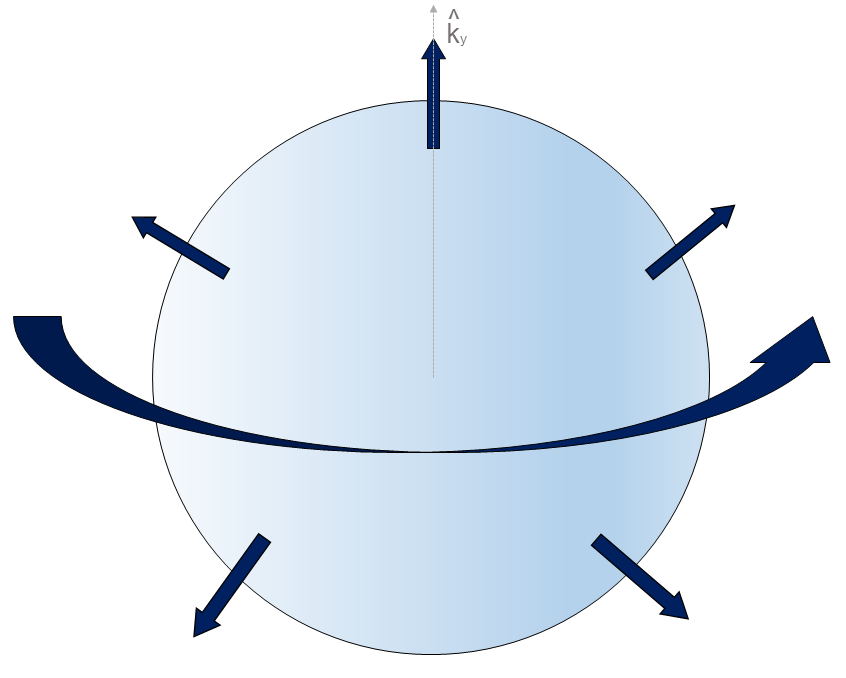
\includegraphics[width=4cm]{model.png}}
	\caption{Modelo de una LAE que se expande y rota.}
	\label{model}
\end{figure}

%Resultados principales y conclusi�n corta
Usando herramientas computacionales, simulo los efectos de velocidad rotacional, velocidad de expansi�n y masa de la LAE en el espectro de salida para diferentes combinaciones de \'estos tres parametros. La conclusi\'on principal es que este nuevo modelo reproduce las caracter\'isticas principales de LAEs observadas. Sin embargo, los ajustes observacionales se dejan para trabajo futuro. Este trabajo de grado, logra el objetivo de extraer la mayor informaci\'on posible de la l\'inea Ly-$\alpha$ de una LAE, con el fin de avanzar nuestro conocimiento sobre esta importante poblaci�n de galaxias. 

%------------------------REFERENCES----------------------------

\bibliographystyle{apj}
\bibliography{references}

\end{document}
%%https://www.modelica.org/events/modelica2014/authors-guide/example-abstract.tex/view